\documentclass{article}

% Language setting
% Replace `english' with e.g. `spanish' to change the document language
\usepackage[english]{babel}

% Set page size and margins
% Replace `letterpaper' with `a4paper' for UK/EU standard size
\usepackage[letterpaper,top=2cm,bottom=2cm,left=2cm,right=2cm,marginparwidth=1.75cm]{geometry}

% Useful packages
\usepackage{amsmath}
\usepackage{graphicx}
\usepackage[colorlinks=true, allcolors=blue]{hyperref}
\providecommand{\e}[1]{\ensuremath{\times 10^{#1}}}

\graphicspath{ {figures/} }

\title{ME469-HW0-UKF-ds0}
\author{Florian Jule}

\begin{document}
\maketitle

\large{Part A}
\normalsize{}

\section{Motion model}

The motion model inputs are: the prior position and orientation: $(x_{t-1}, y_{t-1}, \theta_{t-1})$, the controls input at time $t$, translational and rotational speeds, $(\nu,\omega)$. 
Its outputs are: the posterior estimations of the positions and orientation $(x, y, \theta)$.

We can set a starting position: $(x_0, y_0, \theta_0)$ as a parameter.

This motion model will be used in a UKF. With the UKF, the sigma points will play the role of the state uncertainty, we do not need to introduce additional noise at this stage as we would with other filters.

The robot is assumed to move on a plane, with a given translational and rotational speed over a time step $t$. The robot moves along an arc of circle if $\omega \neq 0$ or in a straight line if $\omega=0$. Below is the derivation of the motion model equations.


Motion model math:
% add plot




This motion model is non linear. The terms $1/\omega, \cos(\theta+\omega t), \sin(\theta+\omega t)$ make it non linear. The  condition where $\omega=0$ is linear.

\section{Motion model test on example commands}
The provided sequence of commands has separate translational and rotational speeds. The robot moves in a successions of straight lines (step 1, 3, 5). The initial state is set to $(0,0,0)$.

\begin{figure}
\centering
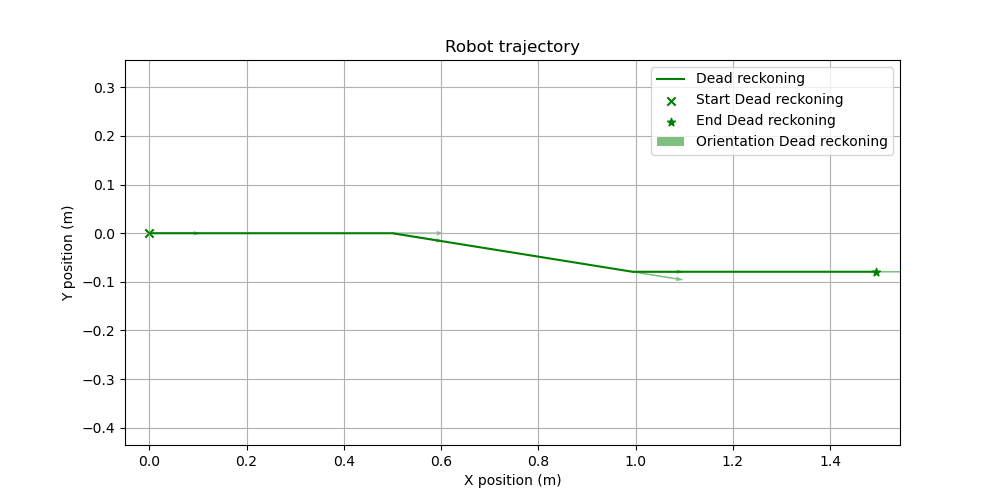
\includegraphics[scale=0.3]{Figure_1.png}
\caption{Robot motion model test on example commands}
\label{fig:figure1}
\end{figure}

\section{Motion model test on robot dataset}
The starting point of the dead-reckoned path uses the ground truth for its initial state. We can observe from \ref{fig:figure2} that the robot is not following the ground truth. The trajectory loosely tracks until it completely diverges after a few turns, every turn introducing more error. We can observe from \ref{fig:figure3} that the robot's position error accumulates over time. After $t=100$, we can see that the y position diverges. For the remainder of the trajectory we can observe an offset between the orientations, that keeps growing over time.
A number of factors can explain this behavior:
\begin{itemize}
      \item The motion model is simple (does not take into account wheel slip for example).
      \item The geometry of the robot could be slightly different from the assumed one (the wheel base has an impact on a differencial drive robot).
      \item The controls could be noisy.
      \item The power unit and drivetrain can have limitations (power limits, acceleration limits).
      \item We assume the speed to be a step function whereas it should be continuous (no infinite acceleration).

\end{itemize}

\begin{figure}
\centering
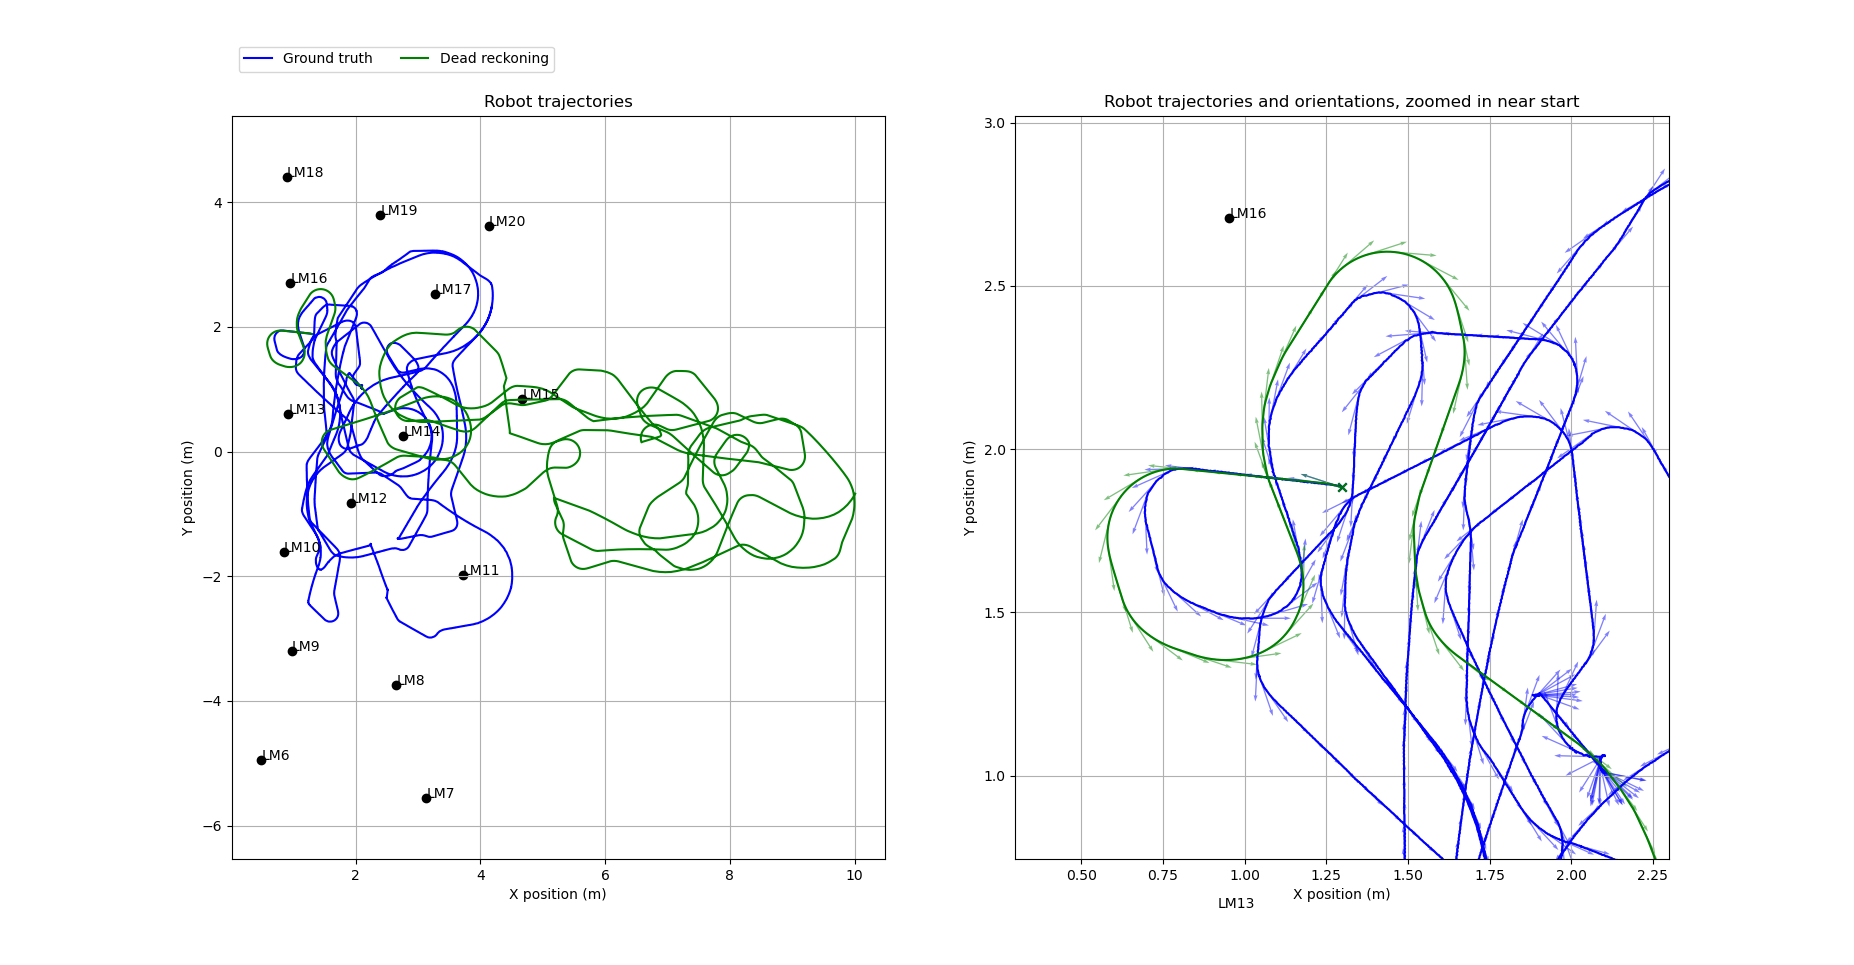
\includegraphics[scale=0.3]{Figure_2.png}
\caption{Robot dead reckoning, compared to ground truth}
\label{fig:figure2}
\end{figure}

\begin{figure}
\centering
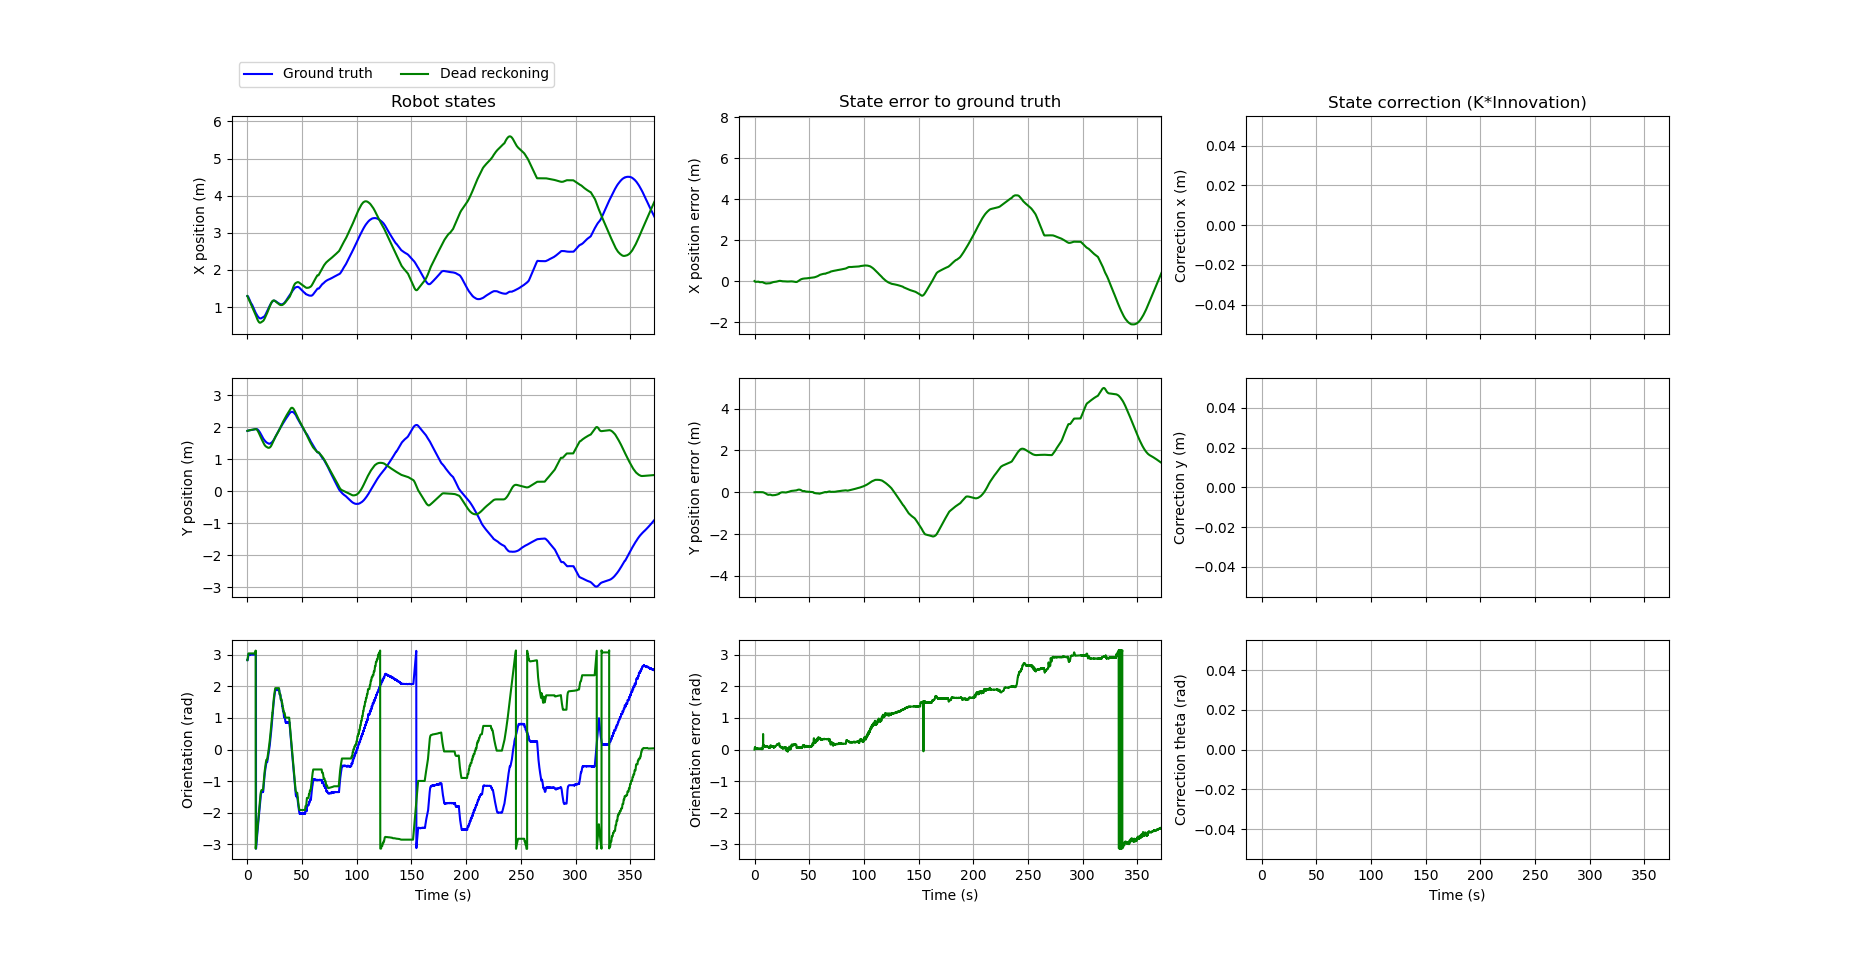
\includegraphics[width=\textwidth]{Figure_3.png}
\caption{Robot position and error}4
\label{fig:figure3}
\end{figure}

\section{Unscented Kalman Filter}

An unscented Kalman filter (UKF) is in concept similar to a Kalman filter, in that unfolds in two steps. The first step is the prediction: it estimates a posterior belief by means of a motion model based on prior state and a control command applied over a time step. The second step is the correction: it uses a measurement model to create an expected measurement of that posterior belief. This is then compared to the actual measurement, and the posterior belief is adjusted based on the difference between expected and actual measurement. Some knowledge of the uncertainty of both model is required for this correction step.

The UKF is different in that it is meant for non-linear models, where the state uncertainty probabilistic parametrisation (gaussian) is not conserved through the model. Instead, the uncertainty is propagated by evaluating sample points (sigma points) through the motion model, and a mean belief and associated covariance is recreated from those points. New sigma points are generated to pass through the measurement model and a mean measurement and associated covariance are constructed. 
% add sigma point math
The remaining algebraic operations are performed on those means (posterior belief and measurement belief).
% Add matrice math here


\section{Measurement model}

The measurement model takes the predicted belief $(x, y, \theta)$ as inputs, as well as knowledge about the space, in this case the measured (assumed true) positions of the landmarks (those are available via the Landmark Groundtruth file).
The model outputs an estimated measurement range and bearing.

The derivation of the measurement model is as follows:
% add math equations and drawing

The measurement data reads landmark barcodes. Those need to be converted to the subject number between 6 and 20 so that they can be paired with the ground truth landmark data. This is done using the barcodes file.


\section{Test of measurement model on robot data}
The measurement model does not add noise and the positions provided are assumed to be the known robot position. The measurement model successfully finds all landmarks with zero error.

\vspace{1cm}
\large{Part B}
\normalsize{}

\section{Filter implementation}

In order for the filter to be implemented on this dataset, some attention needs to be paid to synchronize the data. The controls and the measurements are on different time grids. We interpolate the controls data over a fixed timestep chosen to be 0.05s. This timestep can be updated but seems to have little effects on the overall behavior. The measurements are grouped to the nearest timestep. Because of the lower accuracy of those measurement, this will prove acceptable.

Special attention also needs to be paid when working with angles. Anytime an angle is manipulated, we will normalize it between $]-\pi,\pi]$. We will use the circular mean for means calculations \cite{wiki:circular_mean}.


\section{Comparison to dead reckoning}
Let us look at the data and try to undestand the order of magnitude of the covariance matrices.
Looking at the control data set (resampled at 0.05s intervals), the we find $\nu<0.1m/s$ and $\omega<0.6rad/s$. This means the upper bound a state will evolve after a timestep is $0.005m$ and $0.03rad$. We expect the motion model to be reasonably accurate, we will make an assumption that it is at least 80\% accurate. This means our process noise covariance matrix will have for diagonal elements $\sigma_x^2=\sigma_y^2=(0.005/5)^2=10^{-6},\sigma_\theta^2=(0.03/5)^2=3.6\e{-5}$). We have no data on the measurements accuracy or the robot sensor. It is likely that the measurements are noisy, orders of magnitude higher than the process noise covariance. We will explore this further below when tuning the parameters. For now, we will assume a starting point of $\sigma_{range}^2=0.1^2=10^{-2}, \sigma_{bearing}^2=(6*3.14/180)^2=10^{-2}$.


Now looking at the robot dataset, we can find that the first measurement is collected at $t=11.100s$. Until then, the filter is not providing any correction and the trajectory matches the dead-reckoned path.
However, once the first measurement is collected, the filter starts correcting the trajectory. We can observe from figure 4 that the UKF trajectory mostly tracks the ground truth.

\begin{figure}
\centering
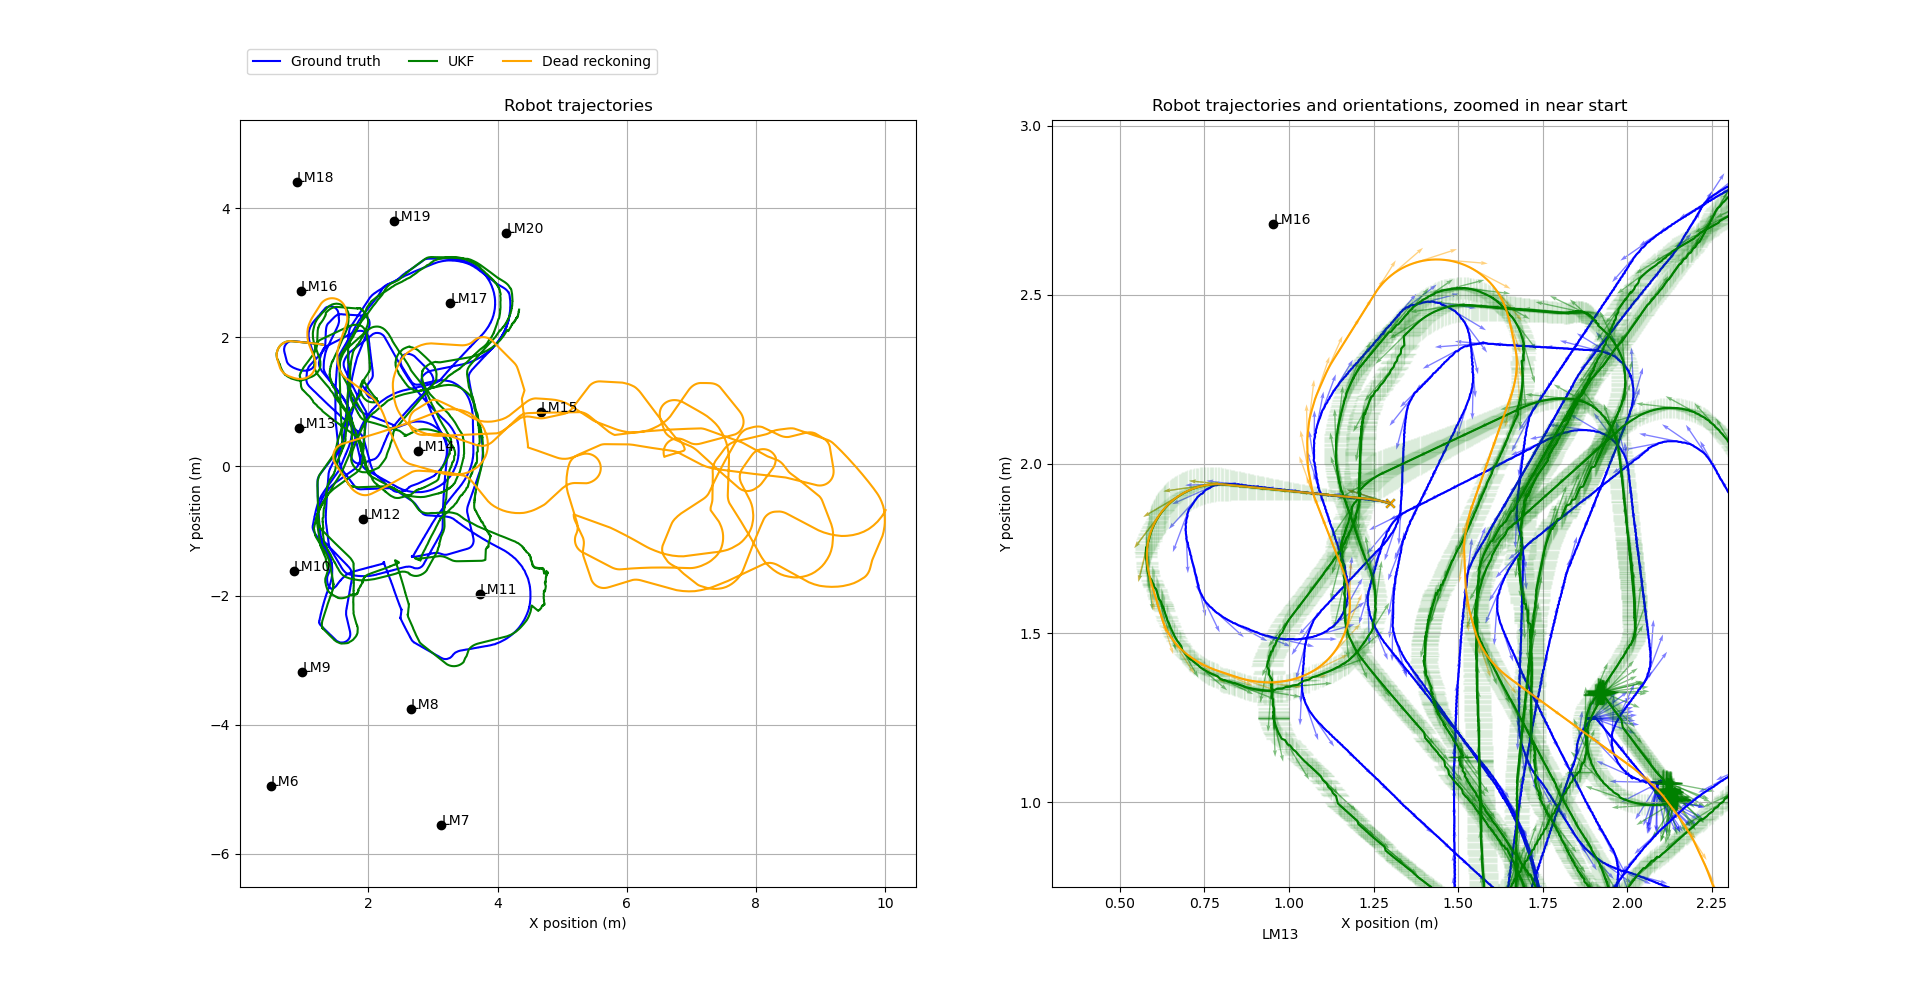
\includegraphics[scale=0.3]{Figure_4.png}
\caption{Robot trajectory predictions with and without UKF. The figure on the right shows the 95 percent confidence interval on position for the UKF trajectory.}
\end{figure}


\begin{figure}
\centering
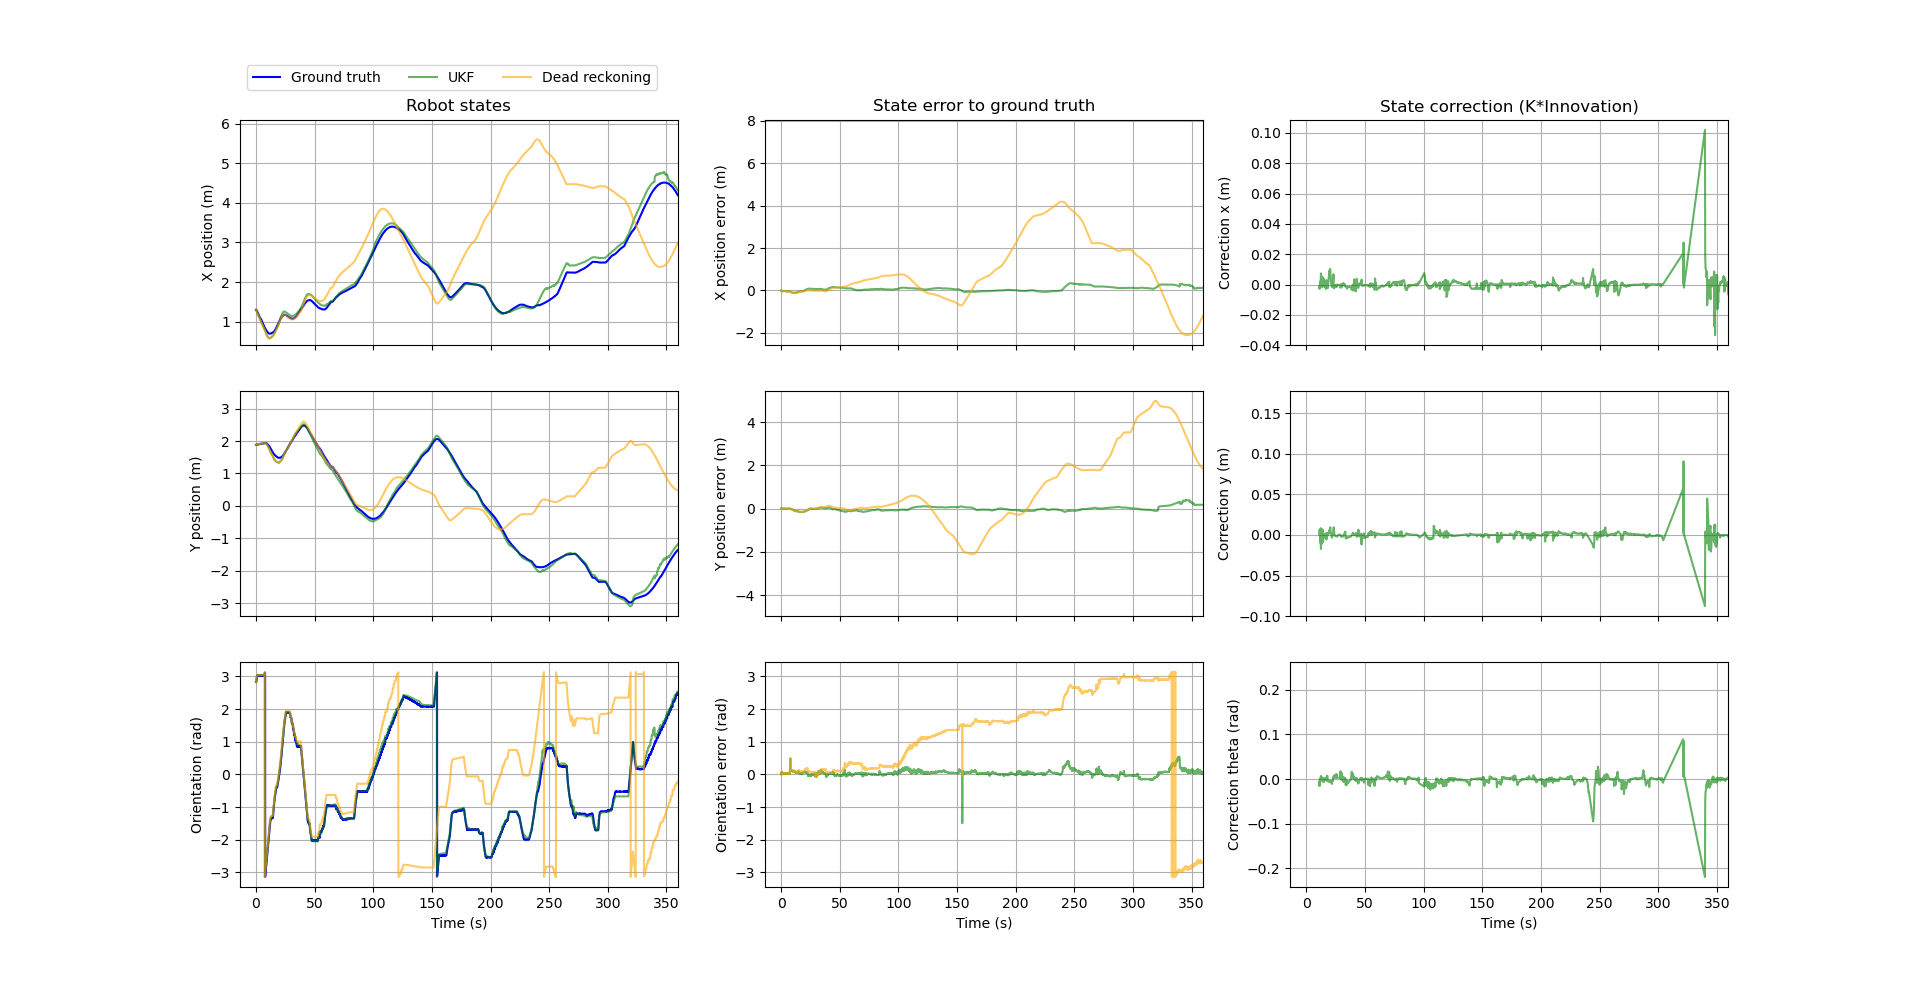
\includegraphics[width=\textwidth]{Figure_5.png}
\caption{Robot states and errors (UKF vs dead reckoning)}
\end{figure}

\section{Filter analysis}
We will in this section perform an exploration of the different filter parameters. We need to be paying attention to the following parameters:
\begin{itemize}
      \item Initial state and its covariance
      \item Process noise covariance
      \item Measurement noise covariance
      \item Alpha
\end{itemize}

We have limited data available on the robot and its controls and sensors, the different covariance matrices (initial state covariance, process noise covariance and measurement noise covariance) have been assumed as diagonal matrices with no inter-dependencies.


\subsection{Process and measurement noise covariance}
With the process noise covariance matrix set to what is believed to be a reasonable value based on the motion model, we can start our exploration on the measurement noise covariance. There is limited knowledge on the sensors being used on the robot.
An estimation of the measurement noise covariance can be estalish iteratively. We will try multiples (1, 0.1, 0.01, 10) of our earlier guess $\sigma_{range}^2=10^{-2}, \sigma_{bearing}^2=10^{-2}$. The plot in \ref{fig:figure6} shows the trajectory predictions for different noise parameters. The plots in \ref{fig:figure7} and \ref{fig:figure8} show the states, errors, predicted measurements and innovations for the different noise parameters. The 95\% confidence interval is shown (defined as +/-2*stddev), to get an idea of the uncertainty of the predictions.

We find, as reported in \ref{fig:figure7} and \ref{fig:figure8}, that the measurement noise covariance has a strong impact on the behavior of the filter. The Kalman gain, which controls how much the posterior is corrected based on the innovation (difference between expected and actual measurement) is directly linked to the ratio between process noise covariance and measurement noise covariance. A higher noise covariance means more uncertainty, and less confidence in the model. The Kalman gain will be higher, and the posterior will be corrected more heavily based on the innovation (and vice versa).

A measurement noise covariance of 5 or more order of magnitude higher than the process noise covariance essentially leads the model to ignore the measurements and leaves the robot dead reckoning.

A measurement noise covariance of the same magnitude as the process noise covariance leads to high overcorrection and very noisy posterior predictions: the position never stabilizes and drifts away from the ground truth. The state is updated with an equivalent control*dt that shows displacement beyond what can be expected reasonable (>2x expected motion).

It seems that a difference in order of magnitude of 4 leads to appreciable results, which is actually consistent with the initial guess. This leads to the smoothest (not over-corrected) and most accurate trajectory. Additionally, one can observe that shifting both the noise covariance higher or lower in pairs has little impact on the trajectory.

\begin{figure}
\centering
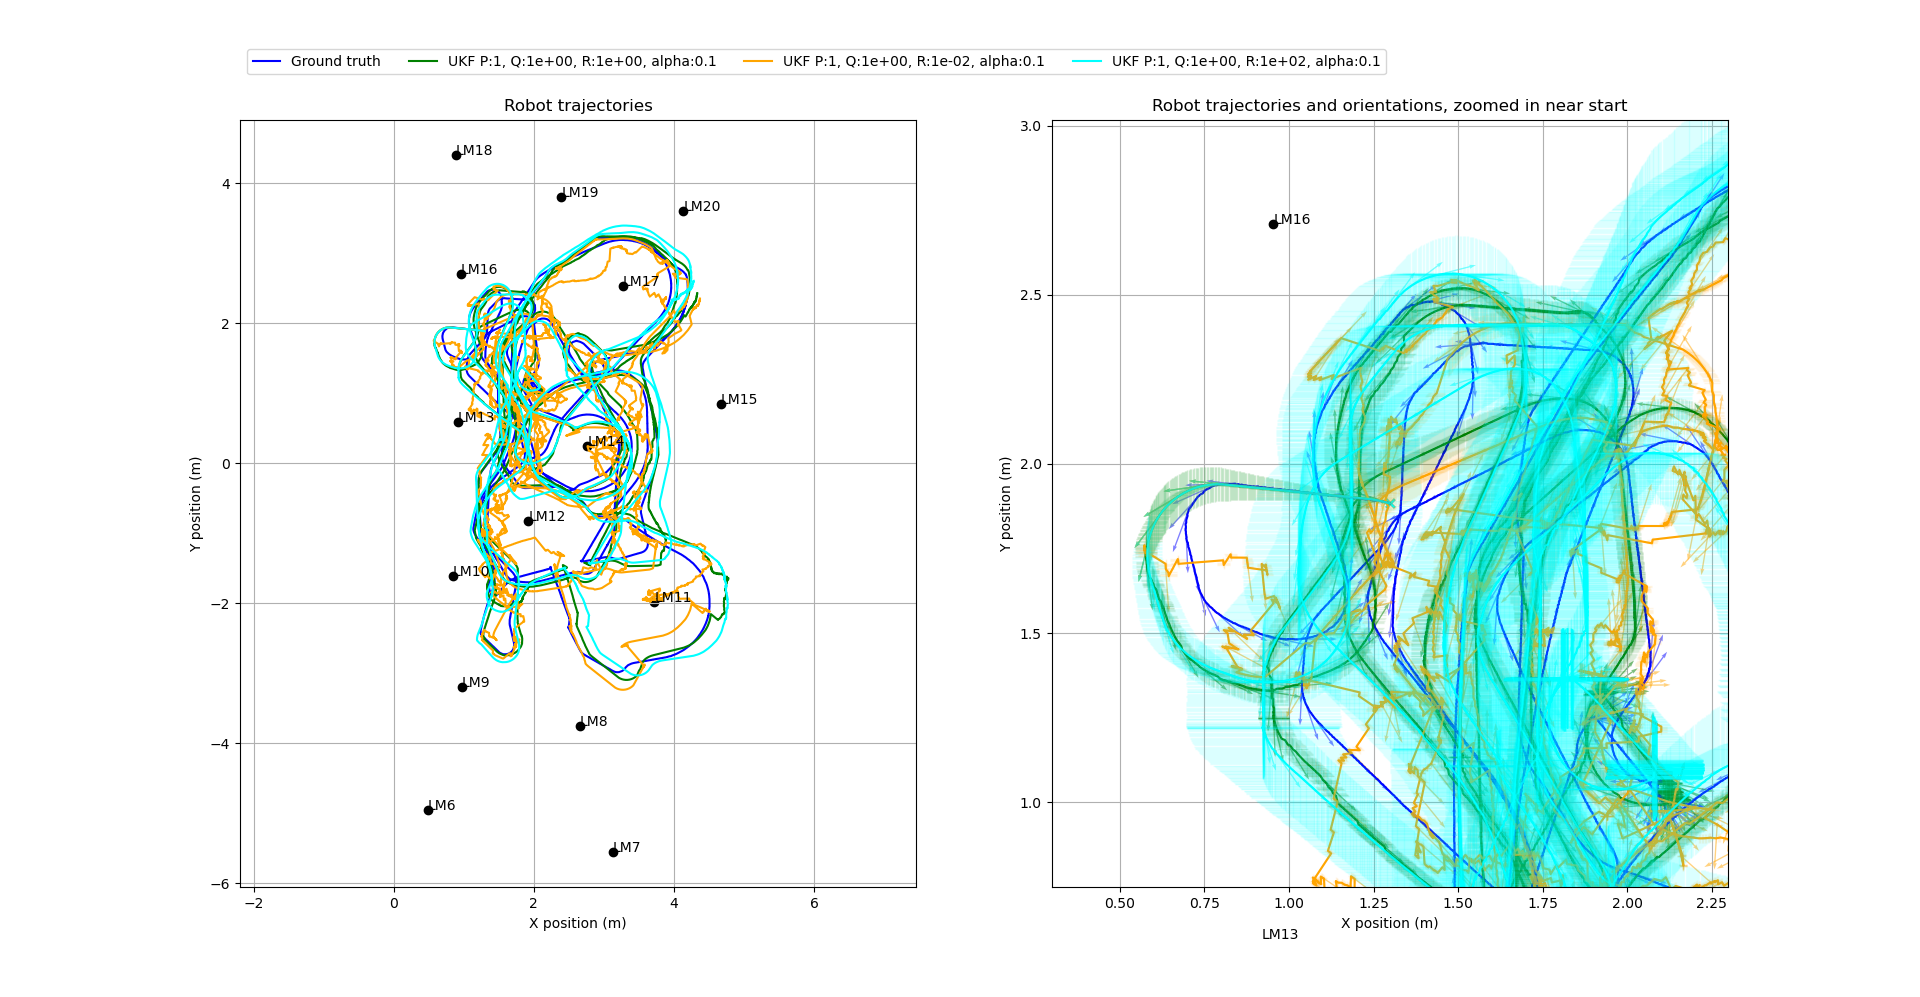
\includegraphics[width=\textwidth]{Figure_6.png}
\caption{Robot trajectory predictions for different UKF noise parameters. The 95 percent confidence interval on position is shown on the right figure.}
\label{fig:figure6}
\end{figure}


\begin{figure}
\centering
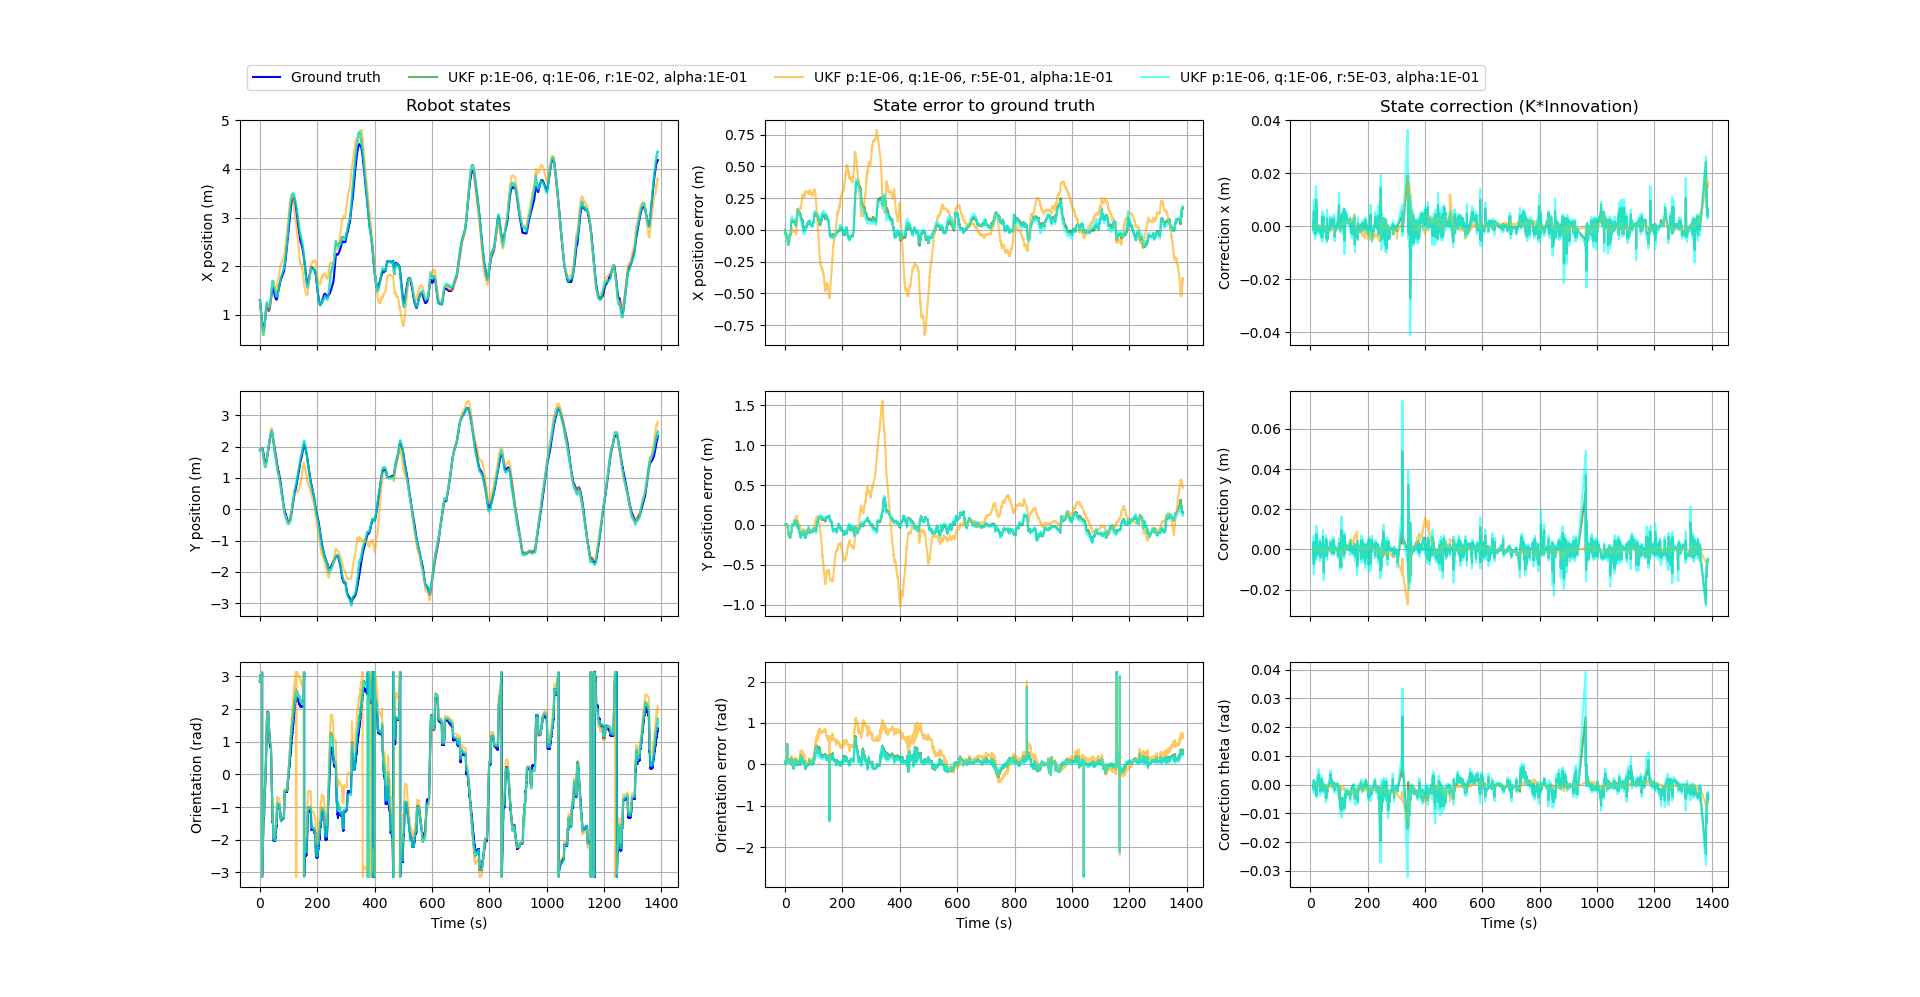
\includegraphics[width=\textwidth]{Figure_7.png}
\caption{Robot states and errors for different UKF noise parameters}
\label{fig:figure7}
\end{figure}

\begin{figure}
\centering
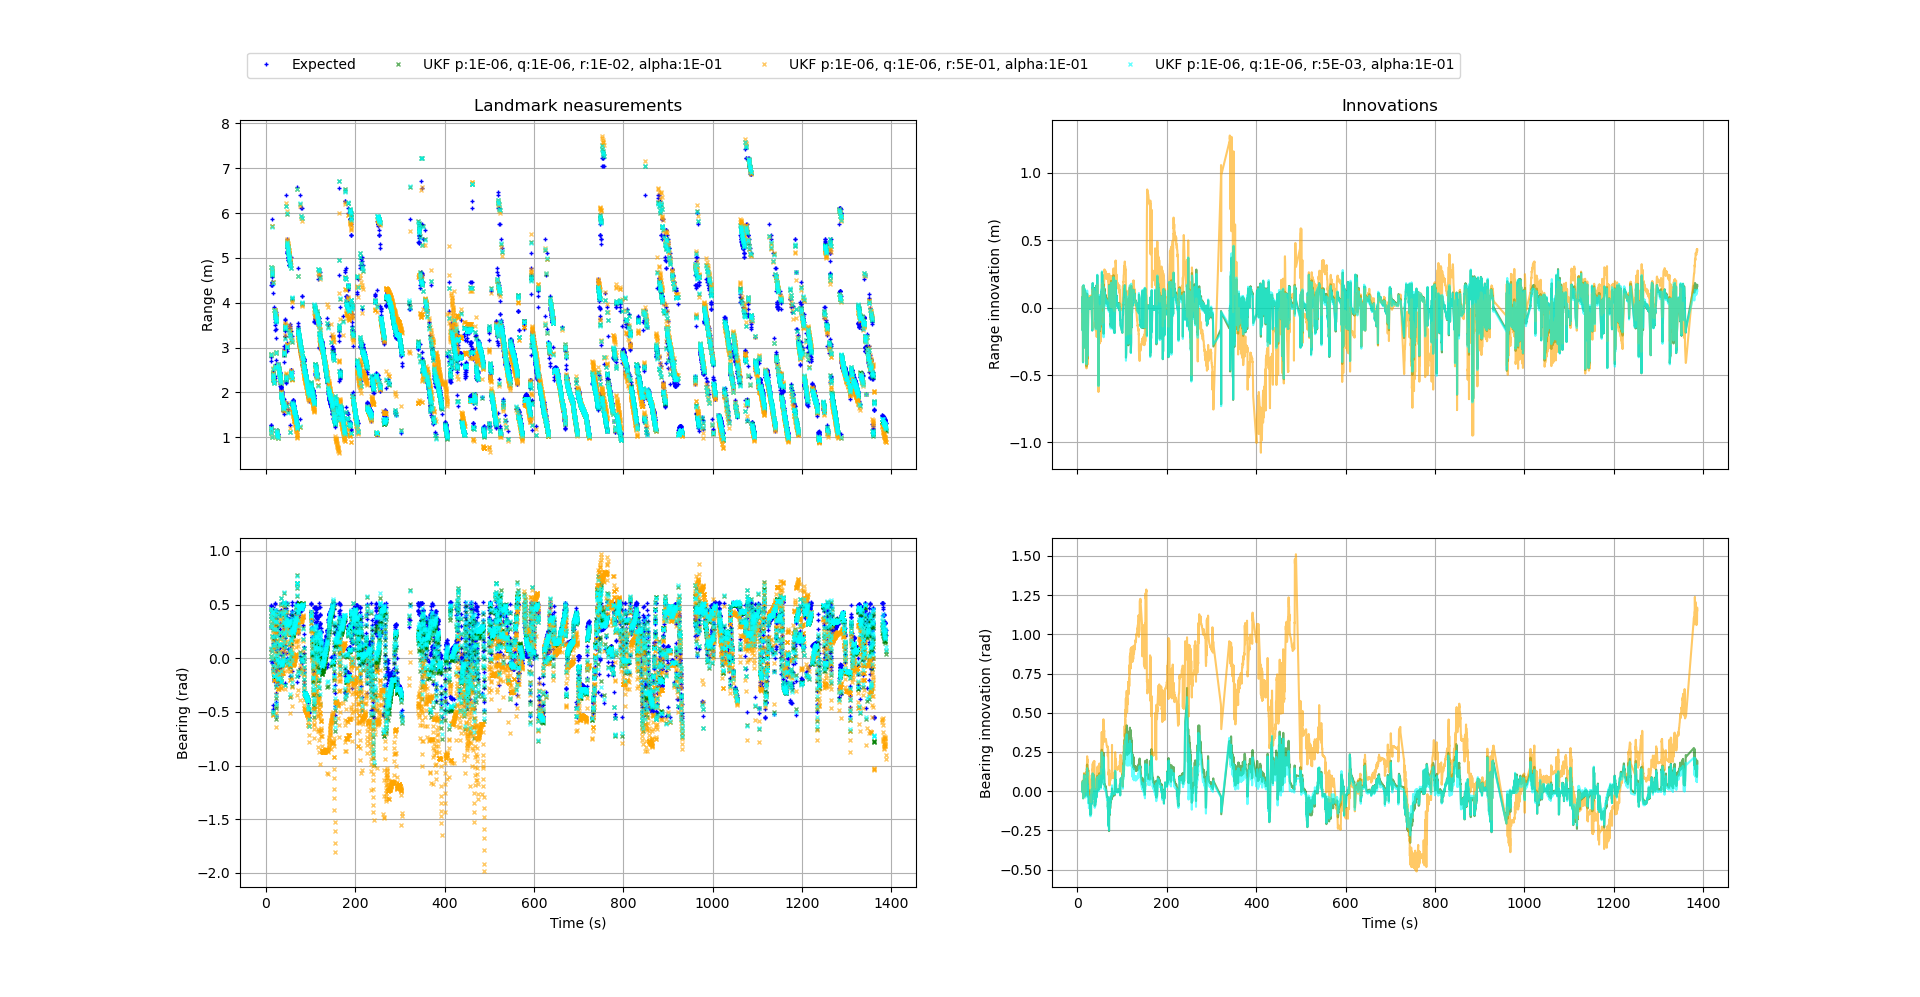
\includegraphics[width=\textwidth]{Figure_8.png}
\caption{Robot predicted measurements and innovations for different UKF noise parameters}
\label{fig:figure8}
\end{figure}

\subsection{Initial state and its covariance}
For a known starting point, the initial state covariance has little to no impact. An initial covariance set fairly high (1e-1) will generate noise, this will however not last and the model corrects this behavior after a few seconds and all estimations become in agreement with one another.
% show plot with different initial cov
% move initial point and check impact on model

\subsection{Alpha}
Alpha controls the spread to the mean when creating the sigma points. After iteratiing for $\alpha=[0.01, 0.1, 1]$, it does not seem to have much of an impact on the behavior of the filter. This gives confidence in the capacity of the sigma points in capturing the non-linear behavior and the assumption about the state estimation as a gaussian (we have a single target / we do not expect a multi modal distribution).

\subsection{Missed measurement}
% find in data longest range with no measurement

\subsection{Multiple measurements}
% find litterature that suggest sequential correction (instead of weighted average)
If several measurements are found for a given time step, the correction step loops over the measurements one by one, using the corrected posterior as the new input for the next measurement.

\subsection{Final considerations}

The initial guess on the process and measurement noise covariance seems to be fairly accurate and no other combination of parameters seems to lead to better results. 


% \section{How to write Mathematics}

% \LaTeX{} is great at typesetting mathematics. Let $X_1, X_2, \ldots, X_n$ be a sequence of independent and identically distributed random variables with $\text{E}[X_i] = \mu$ and $\text{Var}[X_i] = \sigma^2 < \infty$, and let
% \[S_n = \frac{X_1 + X_2 + \cdots + X_n}{n}
%       = \frac{1}{n}\sum_{i}^{n} X_i\]
% denote their mean. Then as $n$ approaches infinity, the random variables $\sqrt{n}(S_n - \mu)$ converge in distribution to a normal $\mathcal{N}(0, \sigma^2)$.


% \bibliographystyle{alpha}
% \bibliography{sample}

\end{document}
